\documentclass[11pt]{report}
\usepackage[abgabe]{protokoll}
\lstset{literate=
  {á}{{\'a}}1 {é}{{\'e}}1 {í}{{\'i}}1 {ó}{{\'o}}1 {ú}{{\'u}}1
  {Á}{{\'A}}1 {É}{{\'E}}1 {Í}{{\'I}}1 {Ó}{{\'O}}1 {Ú}{{\'U}}1
  {à}{{\`a}}1 {è}{{\`e}}1 {ì}{{\`i}}1 {ò}{{\`o}}1 {ù}{{\`u}}1
  {À}{{\`A}}1 {È}{{\'E}}1 {Ì}{{\`I}}1 {Ò}{{\`O}}1 {Ù}{{\`U}}1
  {ä}{{\"a}}1 {ë}{{\"e}}1 {ï}{{\"i}}1 {ö}{{\"o}}1 {ü}{{\"u}}1
  {Ä}{{\"A}}1 {Ë}{{\"E}}1 {Ï}{{\"I}}1 {Ö}{{\"O}}1 {Ü}{{\"U}}1
  {â}{{\^a}}1 {ê}{{\^e}}1 {î}{{\^i}}1 {ô}{{\^o}}1 {û}{{\^u}}1
  {Â}{{\^A}}1 {Ê}{{\^E}}1 {Î}{{\^I}}1 {Ô}{{\^O}}1 {Û}{{\^U}}1
  {œ}{{\oe}}1 {Œ}{{\OE}}1 {æ}{{\ae}}1 {Æ}{{\AE}}1 {ß}{{\ss}}1
  {ű}{{\H{u}}}1 {Ű}{{\H{U}}}1 {ő}{{\H{o}}}1 {Ő}{{\H{O}}}1
  {ç}{{\c c}}1 {Ç}{{\c C}}1 {ø}{{\o}}1 {å}{{\r a}}1 {Å}{{\r A}}1
  {€}{{\EUR}}1 {£}{{\pounds}}1
}
\graphicspath{
  {pictures/}
}
\lstset{inputpath=source/}
\version{0.1$\alpha$}
\datum{\today}

%%
%% Titel, Autor und Betreuer
%%
\fachbereich{VII -- Elektrotechnik - Mechatronik - Optometrie --} 
\studiengang{Elektrotechnik - Schwerpunkt Elektronische Systeme}
\autor{Robby Kozok, Nic Frank Siebenborn, Pascal Kahlert}
\titel{Analog-Digital-Umsetzer und digitale Signale} 
\untertitel{Laborbericht}
\modul{Digitale Signalverarbeitung III}
\betreuerFeld{
  \begin{tabular}{lr}
    \multicolumn{2}{l}{\textbf{Lehrkraft}}\\
    Prof.~Dr.-Ing~Marcus~Purat & Beuth Hochschule für Technik\\
  \end{tabular}
}
%%
%% Abkürzungen
%%
\makenoidxglossaries

\newacronym{isr}{ISR}{Interrupt Service Routine}
\newacronym{pf}{PF}{Programmable Flag}
\newacronym{vi}{VI}{Virtual Instrument}
\newacronym{evb}{EVB}{Evaluationboard}

%%
%% Sourcefile Lising Macro
%%
\makeatletter
\def\app@exe{\immediate\write18}
\def\listDir#1{%
  \app@exe{ls #1/* | xargs cat >> \jobname.tmp}%
  \lstinputlisting{\jobname.tmp}
  \AtEndDocument{\app@exe{rm -f #1/\jobname.tmp}}}
\makeatother


\begin{document}

\pagestyle{fancy}
%%Titelseite

%% Titelseite
\maketitle
\clearpage

%% Leerseite
\newpage

%\chapter*{Einleitung}

%% Einfügen des genutzten Aufgabenblattes. 
\clearpage
%% Seitenzahlen
\pagenumbering{roman}

%% Inhaltsverzeichnis
\tableofcontents

%% Abbildungsverzeichnis


\pagenumbering{arabic}

\chapter{Einleitung}
Dieses Dokument protokoliert die Ergebnisse und Herangehensweise der Laborübung im Rahmen der Veranstaltung Digitale Signalverarbeitung III Labor. 
Als Vorbereitung auf diese Übung wurde sich theoretisch mit dem ADSPBF561EZ-KIT Lite sowie dem darauf eingesetzten Signalprozessor ADSP-BF561 beschäftigt. 
Außerdem wurden Funktionen in der Programmiersprache C erstellt. Im Folgenden wird auf dieser Vorbereitung aufbauend anhand der Aufgabenstellung der Lösungsweg erörtert.
%%Kapitel
\chapter{Einlesen von Signalen}
Im Ersten Versuch soll der Umgang mit der Software VisualDSP++ erlernt werden. 
Dies geschieht mit einem Projekt, welches die Signale am Eingang des Codec zum 
Ausgang des Codec durchreicht. Diese werden dann am PC visualisiert um den Eingang und des Ausgang vergleichen zu können.\\\par 

Entsprechend der Aufgabenstellung wurde ein Projekt angelegt und der kompilierte Code auf das EVB (Evaluationsboard) übertragen. 
Wir legten entsprechend der Aufgabenstellung ein Signal an den rechten Kanal des ADC1 an. 


\begin{figure}[bp!]
  \centering
    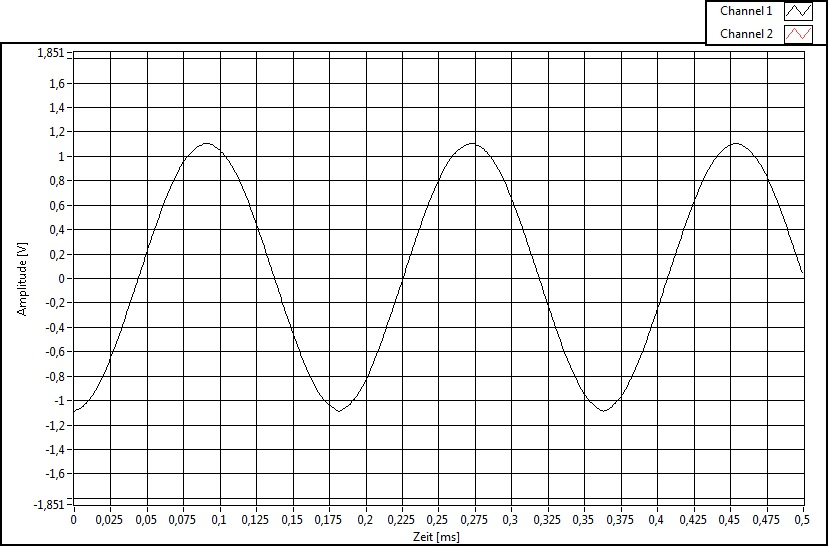
\includegraphics[width=\textwidth]{Aufgabe1Scope1.jpg}
  \caption{Darstellung des Signals am Eingang des Codec.}
  \label{fig:SinusFunktionsGen}
\end{figure}


Dieses Signal wurde, wie alle weiteren mit dem \textit{VI FFT \& FRF \& Scope} 
aufgezeichnet.\pagebreak

In der Vorbereitung wurde die Funktion copyData() erstellt, die sich wie folgt 
aufbaut:
\begin{adjustbox}{width=\textwidth,keepaspectratio}
\lstinputlisting[title=copydata.c]{copydata.c}
\end{adjustbox}

Wie man leicht sieht werden die Werte die der Codec liefert kopiert und in den iDMARxBuffer 
fortlaufend geschrieben, bis dieser voll ist. 
In dem Fall wird an der ersten Position des Buffer erneut angefangen und die alten Werte werden überschrieben.
Software VisualDSP++ biete die Möglichkeit den DSP zu debuggen.\pagebreak


Stoppt man nun den Durchlauf kann man, wie in der Aufgabenstellung beschrieben 
die aktuellen Werte des iDMARxBuffer ausleiten und mit MatLab visualisieren. 
\begin{figure}[!htb]
  \centerline{
    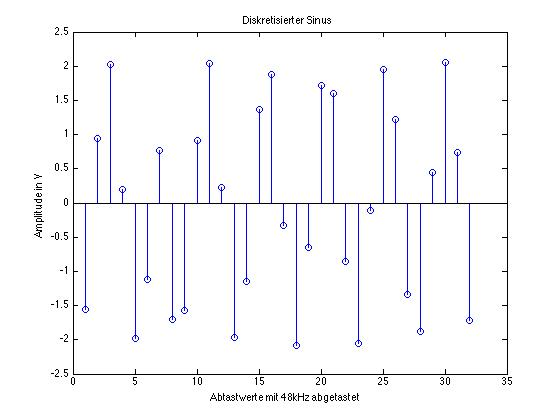
\includegraphics[width=\textwidth]{DiskreterSinusMatlab.jpg}}
      \caption{Darstellung der Datenreihe aus den Werten des DSP.}
      \label{fig:SinusMatlab}
\end{figure}

\section{Auswertung}
Aus Abbildung ~\ref{fig:SinusFunktionsGen} war ein Sinussignal zu erwarten, in Abbildung~\ref{fig:SinusMatlab} ist diese Sinussignal wieder zu erkennen.\\\par
Die Amplitude des Signals beträgt 1446560512 in der Registerdarstellung des DPS. Um diesen Wert exakt ermitteln zu können, wurde die Matlab-Funktion max() 
verwendet
Für die normierte Kreisfrequenz wird der Ansatz 
\begin{equation}\label{normierteKreisfrequenz}
 \omega_0=\frac{2\pi}N 
\end{equation}  

verwendet und führt bei 18 Messwerten in 2 Perioden (es folgt \begin{math}N=\frac{18}{2}\end{math}) zu 
\begin{equation*}
 \omega_0=\frac{2\pi}9 
\end{equation*}

Da die Diskreten Amplitudenwerte im 32-bit-Integer Format vorliegen, müssen sie in eine Spannung umgerechnet werden, hierzu sind die Daten des EVB erforderlich.
Der Codec hat eine Auflösung von 24-bit bei einer Spitze-Spitze-Spannung \begin{math}V_{ss}=6,16V\end{math}.\pagebreak
Es gilt zur Berechnung der Amplitudenspannung \begin{math}V_{Amp}\end{math}
\begin{equation}\label{umrechnungRegisterzuSpannung}
  V_{Amp}=\frac{V_{ADC}*V_{ss}}{2*2^{Registerbreite-1}}
\end{equation} 
Dies ergibt bei einem Registerwert von 1446560512 eine Spannung von 
\begin{math}V_{ss_{max}}=2,0579V\end{math}\\\par
Es ist an dieser Stelle nicht nachweisbar ob es sich bei dem gemessenen Maximalwert auch um das tatsächliche Maximum handelt, 
da der Abtastzeitpunkt nicht unbedingt der Zeitpunkt des lokalen Hochpunktes war.
Auch ist die Frequenz des Ursprungssignals nur näherungsweise zu ermitteln, da die Abtastfrequenz kein ganzzahliges vielfaches der Signalfrequenz ist. 
Um letztgenannten Fehler zu minimieren wurden in erster Annäherung die Abtastwerte über 4 Perioden ermittelt.
Die Frequenz des abgetasteten Sinus lässt sich mit
\begin{equation}\label{freqAbgetastetesSignal}
 f_0=\frac{f_s}N 
\end{equation}  
zu \begin{math}f_0 = 5,3kHz\end{math} berechnen, da der Codec mit 48kHz 
abtastet.\\\par
Aus der Messung ergibt sich grafisch eine Amplitude von \begin{math}V_{ss}=1,1V\end{math} und eine Frequenz von 5,5kHz. 
Die Abweichungen sind u.A. der Messung aus o.g. Gründen und des Ablesens geschuldet. 
Eine weitere Fehlerquelle bildet die interne Schaltung des EVB, so wie der Verstärker zwischen Eingang und ADC.

\chapter{Ausgeben von Signalen}
\chapter{Verarbeiten von Signalen}
\section{Durchf\"uhrung}
Die Aufgabe besteht nun darin, die Signale zu verarbeiten, was hier durch einfaches Verstärken oder Dämpfen realisiert wird.
In einem ersten Schritt wird das eingelesene Signal unverändert über den Codec zurückgegeben. Dies kann mittels \gls{vi} sichtbar gemacht werden. 
Dazu wurde der Funktionsgenerator auf \begin{math}V_{ss} = 1V\end{math} und 500Hz eingestellt, natürlich ergeben sich die üblichen Abweichungen von der tatsächlichen Messung.

\begin{figure}[h!]
  \centering
    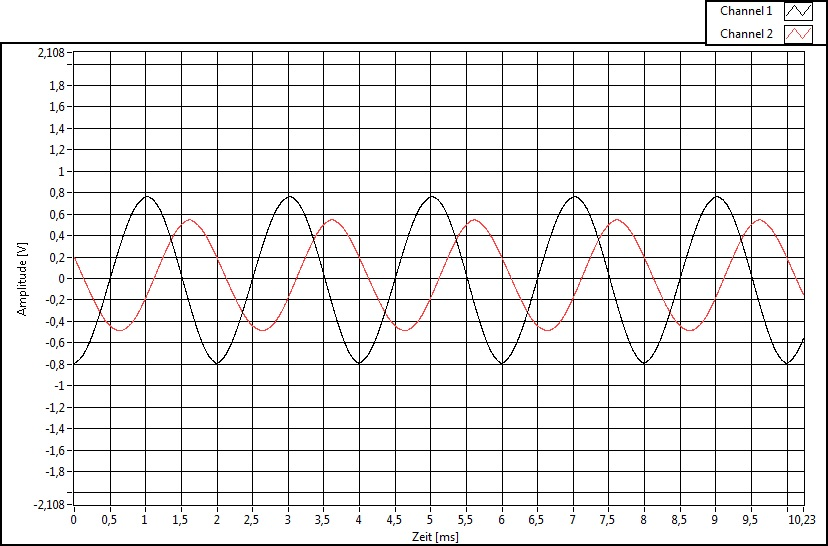
\includegraphics[width=\textwidth]{1V500Hz_ProgrammTest.jpg}
  \caption{Vergleich Eingang und Ausgang in C - 500Hz bei 1V}
  \label{fig:500HzC}
\end{figure}
\begin{figure}[h!]
  \centering
    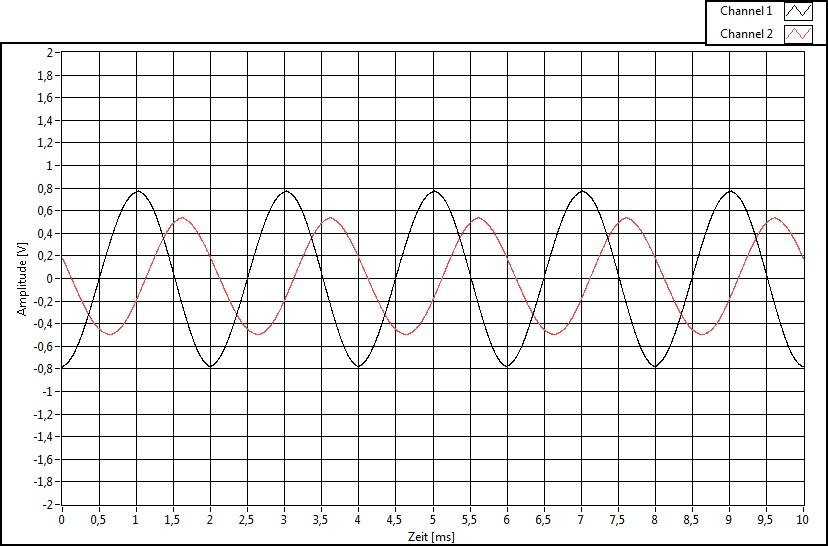
\includegraphics[width=\textwidth]{1V500Hz_AssemblerTest.jpg}
  \caption{Vergleich Eingang und Ausgang in Assembler - 500Hz bei 1V}
  \label{fig:500HzAss}
\end{figure}\pagebreak

Auch wurden die Frequenzgänge und Phasengänge mittels \gls{vi} visualisiert.

\begin{figure}[h!]
  \centering
    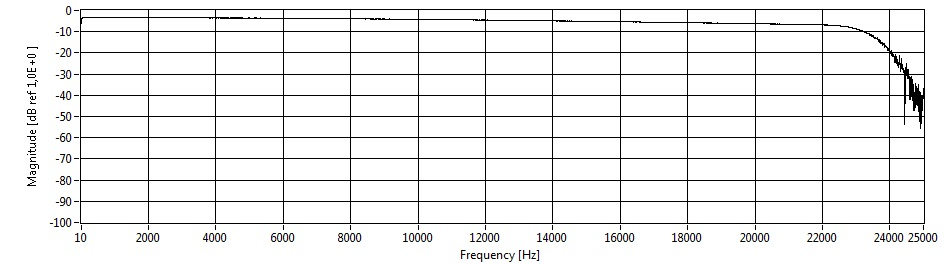
\includegraphics[width=\textwidth]{Frequenzgang_Gesamtsystem.jpg}
  \caption{Frequenzgang Gesamtsystem in C}
  \label{fig:FreqGGesC}
\end{figure}
\begin{figure}[h!]
  \centering
    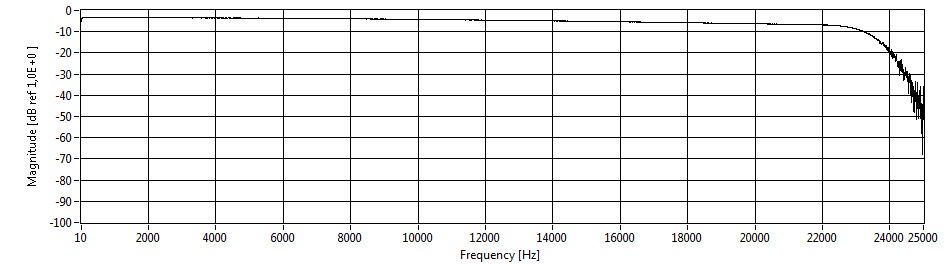
\includegraphics[width=\textwidth]{Frequenzgang_Gesamtsystem_asm.jpg}
  \caption{Frequenzgang Gesamtsystem in Assembler}
  \label{fig:FreqGGesAss}
\end{figure}
\begin{figure}[h!]
  \centering
    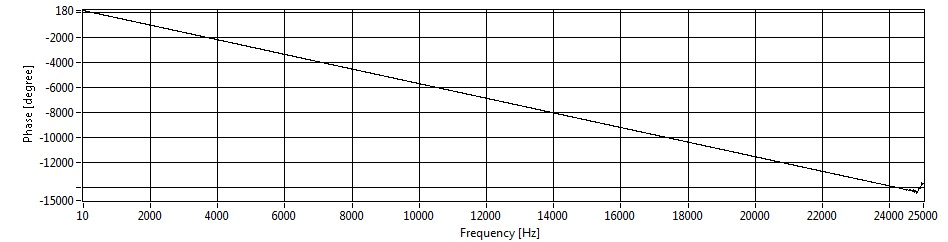
\includegraphics[width=\textwidth]{Phasengang_Gesamtsystem.jpg}
  \caption{Phasengang Gesamtsystem in C}
  \label{fig:PhaGGesC}
\end{figure}
\begin{figure}[h!]
  \centering
    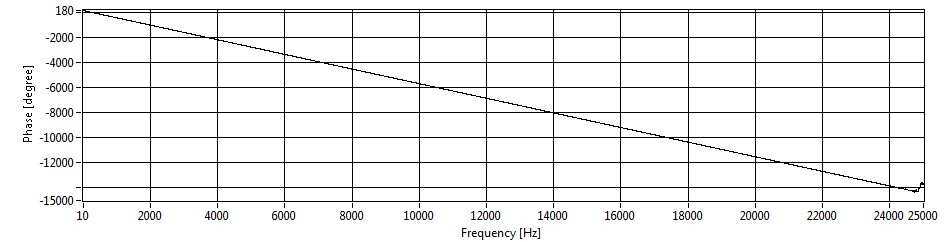
\includegraphics[width=\textwidth]{Phasengang_Gesamtsystem_asm.jpg}
  \caption{Phasengang Gesamtsystem in Assembler}
  \label{fig:PhaGGesAss}
\end{figure}

In Abbildung \ref{fig:500HzC} und Abbildung \ref{fig:500HzAss} ist kein Unterschied sichtbar. Dies entsprach den 
Erwartungen.\pagebreak

Wir haben die Umwandlung der ADC-Werte vom Hexadezimalen in das Signed Integer Format überprüft indem wir im Debugmodus das Programm anhielten und uns die Werte notierten.

\begin{center}
    \begin{tabular}{ | l | l | }\hline
      \multicolumn{2}{|c|}{iADC2R}\\
    \hline
    Hexadezimal & Dezimal \\ \hline
    00d2d300 &	13.881.856,00 \\ \hline
    0038d700 &	14.104.576,00 \\ \hline
    0047d600 &	14.042.880,00 \\ \hline
    00e4d300 &	13.886.464,00 \\ 
    \hline
    \end{tabular}
\end{center}
Es ist zu erkennen, dass das niederwertige Byte stets mit 00h gefüllt ist, 
dies begründet sich darin, dass die 24-bit des Codec stets in die höherwertigen Stellen geschrieben werden.

Im nächsten Schritt wurde das Programm in Assembler auf 16-bit umgestellt, da dies der optimierte Arbeitsbereich des DSP ist.
Hierzu wurde die isr.asm zur isr\textunderscore s.asm mit folgender Änderung entsprechend der 
Aufgabenstellung:\\
 \begin{lstlisting}[title=isr\textunderscore s.asm]{isr_s.asm}
        P1.L = _iDMARxBuffer; 
        P1.H = _iDMARxBuffer;

        R1 = [P1+INTERNAL_ADC_L1*4];
        P2.L = _sADC2L; P2.H = _sADC2L;
        W[P2] = R1.H;//W hinzugefügt um nur die oberen 16-bit zu wählen.
        
        R2 = [P1+INTERNAL_ADC_R1*4];
        P2.L = _sADC2R; P2.H = _sADC2R;
        W[P2] = R2.H;//W hinzugefügt um nur die oberen 16-bit zu wählen.

        P1.L = _iDMATxBuffer; 
        P1.H = _iDMATxBuffer;

        P2.L = _sDAC1L; P2.H = _sDAC1L;
        R1.H = W[P2];//W hinzugefügt um nur die oberen 16-bit zu wählen.
        [P1+INTERNAL_DAC_L0*4] = R1;
        
        P2.L = _sDAC1R; P2.H = _sDAC1R;
        R1.H = W[P2];//W hinzugefügt um nur die oberen 16-bit zu wählen.
        [P1+INTERNAL_DAC_R0*4] = R1;
 \end{lstlisting}

Ein entsprechender Test zeigt, dass keine Veränderung sichtbar wurde.
\begin{figure}[h!]
  \centering
    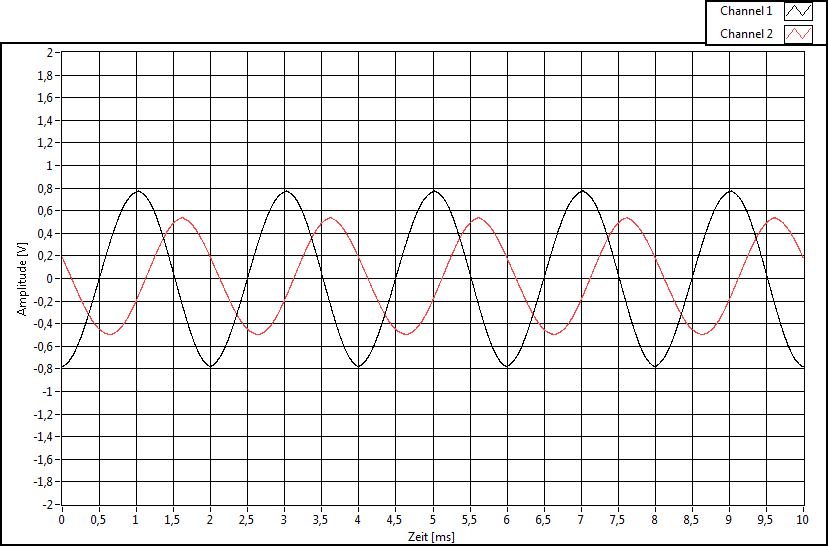
\includegraphics[width=\textwidth]{1V500Hz_AssemblerTest_16Bit.jpg}
  \caption{Vergleich Eingang und Ausgang in C und 16-bit - 500Hz bei 1V}
  \label{fig:500HzC16}
\end{figure}
  
\pagebreak



Der letzte Abschnitt der Aufgabe beinhaltete eine Amplitudenver\"anderung des Signals. Dies wurde in process\textunderscore data\textunderscore s.asm 
bearbeitet.\\
\lstinputlisting[title=processdatas.asm]{processdatas.asm}
Für die einzelnen Tests wurden die entsprechenden Zeilen die nicht genutzt wurden kommentiert. So ist in diesem Beispiel die Variante der Arithmetischen Division durch vier zu sehen.
\section{Auswertung}
In den folgenden Bildern ist das Originalsignal in schwarz und das \gls{evb}-Ausgangssignal mit Verzögerung und Amplitudenver\"anderung zu 
erkennen.\pagebreak

\begin{figure}[h!]
  \centering
    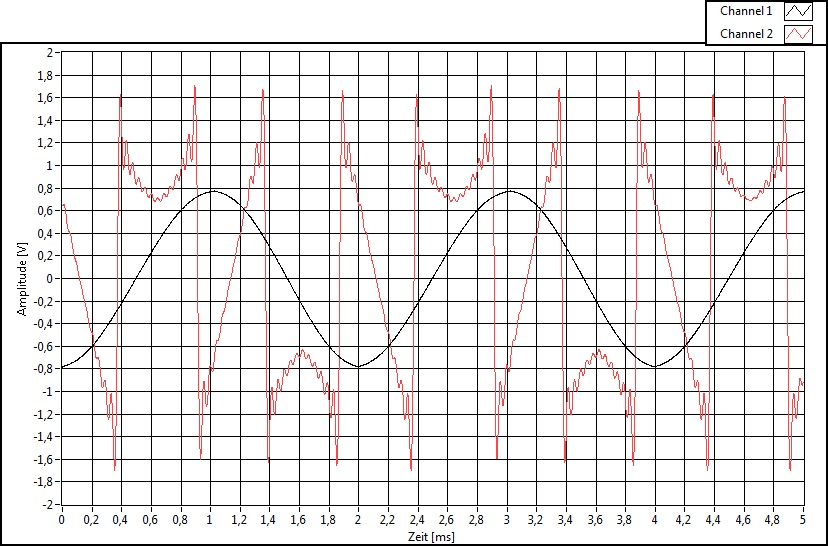
\includegraphics[width=\textwidth]{Mul4_ohneS.jpg}
  \caption{Multiplikation mit 4 ohne Sättigung}
  \label{fig:Mul4_ohneS}
\end{figure}
In Abbildung \ref{fig:Mul4_ohneS} ist ein \"Uberlaufverhalten zu erkennen, welches zu entsprechenden Fehlern führt. Außerdem ist dem Signal ein Rauschen 
überlagert.

\begin{figure}[h!]
  \centering
    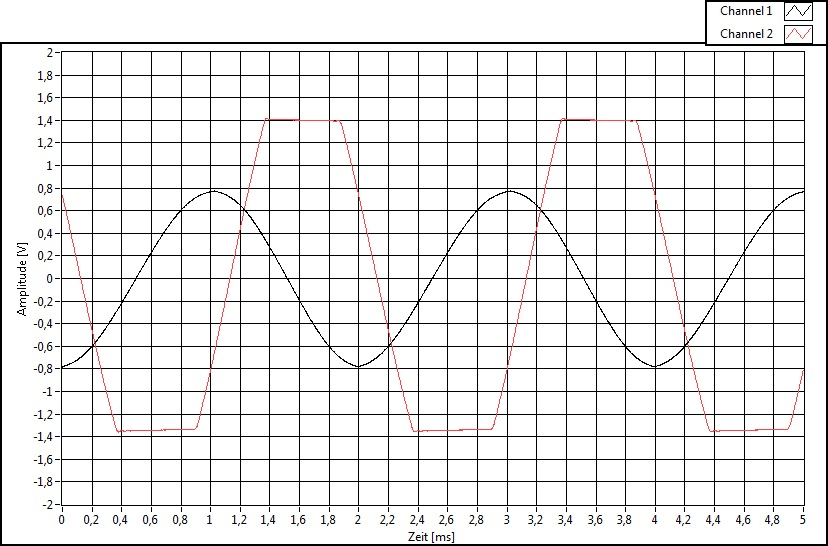
\includegraphics[width=\textwidth]{Mul4_mitS.jpg}
  \caption{Multiplikation mit 4 mit Sättigung}
  \label{fig:Mul4_mitS}
\end{figure}

Im Unterschied zur Abbildung \ref{fig:Mul4_ohneS} ist in Abbildung \ref{fig:Mul4_mitS} zu sehen, dass es zu keinen reinen Überläufen kommt, sondern der maximale Aussteuerungsbereich verwendet wird.
Dies führt zu geringeren Fehlern, allerdings ist der originale Signalverlauf nicht rekonstruierbar, da die Maxima nicht mehr sichtbar sind.
\begin{figure}[b!]
  \centering
    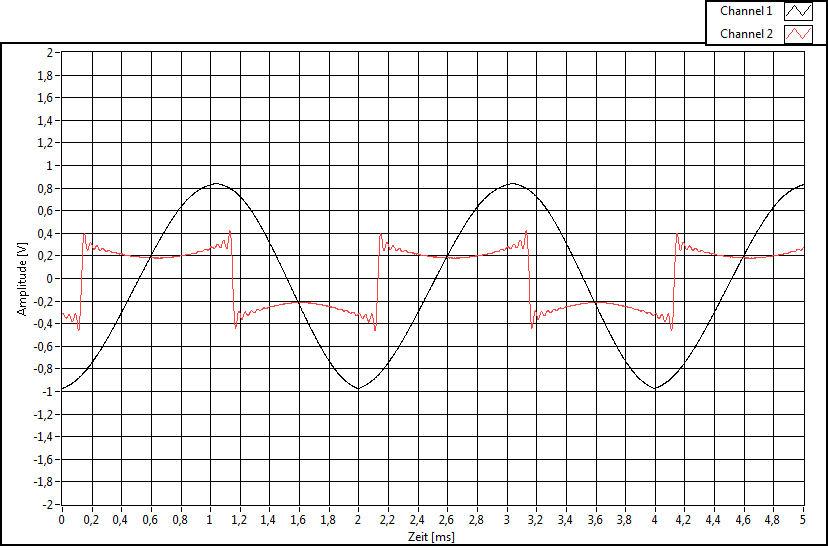
\includegraphics[width=\textwidth]{divlog.png}
  \caption{Logische Division mit 4}
  \label{fig:divlog}
\end{figure}
Der  logische  Shift  sorgt  f\"ur  den  Verlust  des  Vorzeichens,  was  zu  rein  positiven  Werten
f\"uhrt, da immer eine 0 nachgeschoben wird. 
Es sind nicht nur positive Werte zu sehen, da dieser Gleichanteil durch die Gleichspanungsentkopplung des Codes gefiltert wird.
Die Verringerung der Amplitude ist trotzdem zu sehen. 
Der arithmetische Shift verändert das Vorzeichen des Signals nicht und ermöglicht es den Signalverlauf beizubehalten. 
Lediglich die \"Anderung der Amplitude macht sich bemerkbar.
\begin{figure}[h!]
  \centering
    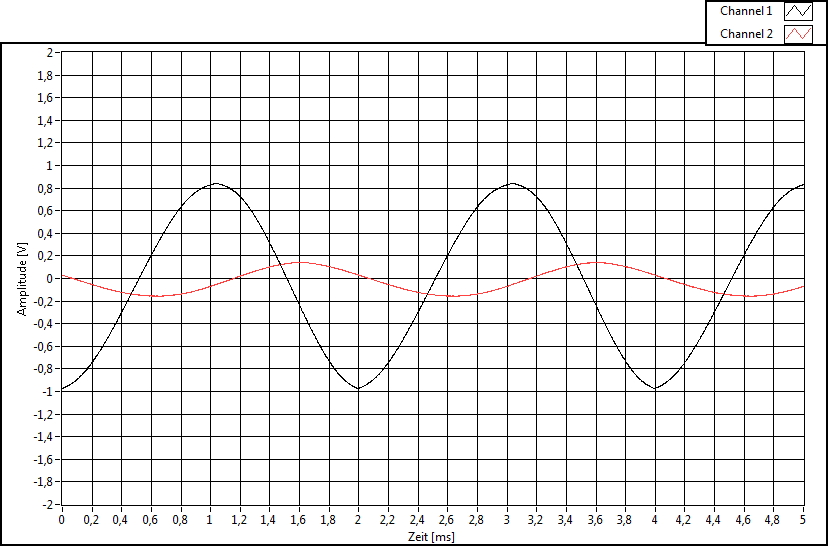
\includegraphics[width=\textwidth]{divarith.png}
  \caption{Arithmetische Division mit 4}
  \label{fig:divarith}
\end{figure}

Der arithmetische Shift behält stets sein Vorzeichen und ermöglicht daher das Signal beizubehalten und lediglich die \"Anderung der Amplitude macht sich 
bemerkbar.\\\par \pagebreak
Die Signallaufzeit lässt sich mit Hilfe des Phasenganges Graphisch ermitteln. 
In Abbildung \ref{fig:PhaGGesAss} und Abbildung \ref{fig:PhaGGesC} ist eine Phasenverschiebung -8000° bei 14kHz zu erkennen. Dies entspricht etwa 22 
Perioden.\\\par
Gemäß \begin{math}\frac{22}{14kHz} = 1,6ms\end{math} ergibt sich eine Laufzeit von 1,6ms. 
Diese Zeit resultiert zum einen aus der Verarbeitung durch die Software, aber auch durch die Wandlungen des Codec, wobei die Wandlungen den größten Anteil haben dürften. 
Ein weiterer Teil der Verzögerung wird dadurch verursacht, dass zwischen Ermitteln der Werte des ADC und Ablegen dieser im Speicher ein Taktzyklus liegt.

%Bitte alle code dateien die wir bearbeitet ahben anhängen


%%Anhang
\begin{appendix}
  \chapter{Quelltext-Dateien}




\end{appendix}

\clearpage\newpage
\listoffigures

\printnoidxglossary[type=\acronymtype,title=Abkürzungsverzeichnis]

\end{document}